\documentclass[a4paper]{article}

\usepackage[pdftex,
  hidelinks,
  pdfauthor={Dexter Chua},
  pdfsubject={Cambridge Maths Notes: Part IB - Optimisation},
  pdftitle={Part IB - Optimisation},
pdfkeywords={Cambridge Mathematics Maths Math IB Easter Optimisation}]{hyperref}

\title{Part IB - Optimisation}
\author{Lectured by F. A. Fischer}
\date{Easter 2015}

% Imports
\ifx \nextra \undefined
  \usepackage[pdftex,
    hidelinks,
    pdfauthor={Dexter Chua},
    pdfsubject={Cambridge Maths Notes: Part \npart\ - \ncourse},
    pdftitle={Part \npart\ - \ncourse},
  pdfkeywords={Cambridge Mathematics Maths Math \npart\ \nterm\ \nyear\ \ncourse}]{hyperref}
  \title{Part \npart\ - \ncourse}
\else
  \usepackage[pdftex,
    hidelinks,
    pdfauthor={Dexter Chua},
    pdfsubject={Cambridge Maths Notes: Part \npart\ - \ncourse\ (\nextra)},
    pdftitle={Part \npart\ - \ncourse\ (\nextra)},
  pdfkeywords={Cambridge Mathematics Maths Math \npart\ \nterm\ \nyear\ \ncourse\ \nextra}]{hyperref}

  \title{Part \npart\ - \ncourse \\ {\Large \nextra}}
\fi

\author{Lectured by \nlecturer \\\small Notes taken by Dexter Chua}
\date{\nterm\ \nyear}

\usepackage{alltt}
\usepackage{amsfonts}
\usepackage{amsmath}
\usepackage{amssymb}
\usepackage{amsthm}
\usepackage{booktabs}
\usepackage{caption}
\usepackage{enumitem}
\usepackage{fancyhdr}
\usepackage{graphicx}
\usepackage{mathtools}
\usepackage{microtype}
\usepackage{multirow}
\usepackage{pdflscape}
\usepackage{pgfplots}
\usepackage{siunitx}
\usepackage{tabularx}
\usepackage{tikz}
\usepackage{tkz-euclide}
\usepackage[normalem]{ulem}
\usepackage[all]{xy}

\pgfplotsset{compat=1.12}

\pagestyle{fancyplain}
\lhead{\emph{\nouppercase{\leftmark}}}
\ifx \nextra \undefined
  \rhead{
    \ifnum\thepage=1
    \else
      \npart\ \ncourse
    \fi}
\else
  \rhead{
    \ifnum\thepage=1
    \else
      \npart\ \ncourse\ (\nextra)
    \fi}
\fi
\usetikzlibrary{arrows}
\usetikzlibrary{decorations.markings}
\usetikzlibrary{decorations.pathmorphing}
\usetikzlibrary{positioning}
\usetikzlibrary{fadings}
\usetikzlibrary{intersections}
\usetikzlibrary{cd}

\newcommand*{\Cdot}{\raisebox{-0.25ex}{\scalebox{1.5}{$\cdot$}}}
\newcommand {\pd}[2][ ]{
  \ifx #1 { }
    \frac{\partial}{\partial #2}
  \else
    \frac{\partial^{#1}}{\partial #2^{#1}}
  \fi
}

% Theorems
\theoremstyle{definition}
\newtheorem*{aim}{Aim}
\newtheorem*{axiom}{Axiom}
\newtheorem*{claim}{Claim}
\newtheorem*{cor}{Corollary}
\newtheorem*{defi}{Definition}
\newtheorem*{eg}{Example}
\newtheorem*{fact}{Fact}
\newtheorem*{law}{Law}
\newtheorem*{lemma}{Lemma}
\newtheorem*{notation}{Notation}
\newtheorem*{prop}{Proposition}
\newtheorem*{thm}{Theorem}

\renewcommand{\labelitemi}{--}
\renewcommand{\labelitemii}{$\circ$}
\renewcommand{\labelenumi}{(\roman{*})}

\let\stdsection\section
\renewcommand\section{\newpage\stdsection}

% Strike through
\def\st{\bgroup \ULdepth=-.55ex \ULset}

% Maths symbols
\newcommand{\bra}{\langle}
\newcommand{\ket}{\rangle}

\newcommand{\N}{\mathbb{N}}
\newcommand{\Z}{\mathbb{Z}}
\newcommand{\Q}{\mathbb{Q}}
\renewcommand{\H}{\mathbb{H}}
\newcommand{\R}{\mathbb{R}}
\newcommand{\C}{\mathbb{C}}
\newcommand{\Prob}{\mathbb{P}}
\renewcommand{\P}{\mathbb{P}}
\newcommand{\E}{\mathbb{E}}
\newcommand{\F}{\mathbb{F}}
\newcommand{\cU}{\mathcal{U}}
\newcommand{\RP}{\mathbb{RP}}
\newcommand{\CP}{\mathbb{CP}}

\newcommand{\ph}{\,\cdot\,}

\DeclareMathOperator{\sech}{sech}
\DeclareMathOperator{\cosech}{cosech}
\DeclareMathOperator{\cosec}{cosec}

\DeclareMathOperator{\covol}{covol}
\DeclareMathOperator{\vol}{vol}

\let\Im\relax
\let\Re\relax
\DeclareMathOperator{\Im}{Im}
\DeclareMathOperator{\Re}{Re}
\DeclareMathOperator{\im}{im}
\DeclareMathOperator{\image}{image}
\DeclareMathOperator{\Ann}{Ann}

\DeclareMathOperator*{\res}{res}
\DeclareMathOperator{\Res}{Res}
\DeclareMathOperator{\Ind}{Ind}

\DeclareMathOperator{\tr}{tr}
\DeclareMathOperator{\diag}{diag}
\DeclareMathOperator{\rank}{rank}
\DeclareMathOperator{\card}{card}
\DeclareMathOperator{\spn}{span}
\DeclareMathOperator{\adj}{adj}

\DeclareMathOperator{\erf}{erf}
\DeclareMathOperator{\erfc}{erfc}

\DeclareMathOperator{\ord}{ord}
\DeclareMathOperator{\Sym}{Sym}

\DeclareMathOperator{\sgn}{sgn}
\DeclareMathOperator{\orb}{orb}
\DeclareMathOperator{\stab}{stab}
\DeclareMathOperator{\ccl}{ccl}

\DeclareMathOperator{\lcm}{lcm}
\DeclareMathOperator{\hcf}{hcf}

\DeclareMathOperator{\Int}{Int}
\DeclareMathOperator{\id}{id}

\DeclareMathOperator{\betaD}{beta}
\DeclareMathOperator{\gammaD}{gamma}
\DeclareMathOperator{\Poisson}{Poisson}
\DeclareMathOperator{\binomial}{binomial}
\DeclareMathOperator{\multinomial}{multinomial}
\DeclareMathOperator{\Bernoulli}{Bernoulli}
\DeclareMathOperator{\like}{like}

\DeclareMathOperator{\var}{var}
\DeclareMathOperator{\cov}{cov}
\DeclareMathOperator{\bias}{bias}
\DeclareMathOperator{\mse}{mse}
\DeclareMathOperator{\corr}{corr}

\DeclareMathOperator{\otp}{otp}
\DeclareMathOperator{\dom}{dom}

\DeclareMathOperator{\Root}{Root}
\DeclareMathOperator{\supp}{supp}
\DeclareMathOperator{\rel}{rel}
\DeclareMathOperator{\Hom}{Hom}
\DeclareMathOperator{\Aut}{Aut}
\DeclareMathOperator{\Gal}{Gal}
\DeclareMathOperator{\Mat}{Mat}
\DeclareMathOperator{\End}{End}
\DeclareMathOperator{\Char}{char}
\DeclareMathOperator{\ev}{ev}
\DeclareMathOperator{\St}{St}
\DeclareMathOperator{\Lk}{Lk}
\DeclareMathOperator{\disc}{disc}
\DeclareMathOperator{\Isom}{Isom}
\DeclareMathOperator{\length}{length}
\DeclareMathOperator{\energy}{energy}
\DeclareMathOperator{\area}{area}
\DeclareMathOperator{\Syl}{Syl}
\DeclareMathOperator{\cl}{cl}
\DeclareMathOperator{\fix}{fix}

\newcommand{\GL}{\mathrm{GL}}
\newcommand{\SL}{\mathrm{SL}}
\newcommand{\PGL}{\mathrm{PGL}}
\newcommand{\PSL}{\mathrm{PSL}}
\newcommand{\PSU}{\mathrm{PSU}}
\newcommand{\Or}{\mathrm{O}}
\newcommand{\SO}{\mathrm{SO}}
\newcommand{\U}{\mathrm{U}}
\newcommand{\SU}{\mathrm{SU}}

\renewcommand{\d}{\mathrm{d}}
\newcommand{\D}{\mathrm{D}}

\tikzset{->/.style = {decoration={markings,
                                  mark=at position 1 with {\arrow[scale=2]{latex'}}},
                      postaction={decorate}}}
\tikzset{<-/.style = {decoration={markings,
                                  mark=at position 0 with {\arrowreversed[scale=2]{latex'}}},
                      postaction={decorate}}}
\tikzset{<->/.style = {decoration={markings,
                                   mark=at position 0 with {\arrowreversed[scale=2]{latex'}},
                                   mark=at position 1 with {\arrow[scale=2]{latex'}}},
                       postaction={decorate}}}
\tikzset{->-/.style = {decoration={markings,
                                   mark=at position #1 with {\arrow[scale=2]{latex'}}},
                       postaction={decorate}}}
\tikzset{-<-/.style = {decoration={markings,
                                   mark=at position #1 with {\arrowreversed[scale=2]{latex'}}},
                       postaction={decorate}}}

\tikzset{circ/.style = {fill, circle, inner sep = 0, minimum size = 3}}
\tikzset{mstate/.style={circle, draw, blue, text=black, minimum width=0.7cm}}

\definecolor{mblue}{rgb}{0.2, 0.3, 0.8}
\definecolor{morange}{rgb}{1, 0.5, 0}
\definecolor{mgreen}{rgb}{0.1, 0.4, 0.2}
\definecolor{mred}{rgb}{0.5, 0, 0}

\def\drawcirculararc(#1,#2)(#3,#4)(#5,#6){%
    \pgfmathsetmacro\cA{(#1*#1+#2*#2-#3*#3-#4*#4)/2}%
    \pgfmathsetmacro\cB{(#1*#1+#2*#2-#5*#5-#6*#6)/2}%
    \pgfmathsetmacro\cy{(\cB*(#1-#3)-\cA*(#1-#5))/%
                        ((#2-#6)*(#1-#3)-(#2-#4)*(#1-#5))}%
    \pgfmathsetmacro\cx{(\cA-\cy*(#2-#4))/(#1-#3)}%
    \pgfmathsetmacro\cr{sqrt((#1-\cx)*(#1-\cx)+(#2-\cy)*(#2-\cy))}%
    \pgfmathsetmacro\cA{atan2(#2-\cy,#1-\cx)}%
    \pgfmathsetmacro\cB{atan2(#6-\cy,#5-\cx)}%
    \pgfmathparse{\cB<\cA}%
    \ifnum\pgfmathresult=1
        \pgfmathsetmacro\cB{\cB+360}%
    \fi
    \draw (#1,#2) arc (\cA:\cB:\cr);%
}
\newcommand\getCoord[3]{\newdimen{#1}\newdimen{#2}\pgfextractx{#1}{\pgfpointanchor{#3}{center}}\pgfextracty{#2}{\pgfpointanchor{#3}{center}}}

\def\Xint#1{\mathchoice
   {\XXint\displaystyle\textstyle{#1}}%
   {\XXint\textstyle\scriptstyle{#1}}%
   {\XXint\scriptstyle\scriptscriptstyle{#1}}%
   {\XXint\scriptscriptstyle\scriptscriptstyle{#1}}%
   \!\int}
\def\XXint#1#2#3{{\setbox0=\hbox{$#1{#2#3}{\int}$}
     \vcenter{\hbox{$#2#3$}}\kern-.5\wd0}}
\def\ddashint{\Xint=}
\def\dashint{\Xint-}


\begin{document}
\maketitle
{\small
\noindent\textbf{Lagrangian methods}\\
General formulation of constrained problems; the Lagrangian sufficiency theorem.  Interpretation of Lagrange multipliers as shadow prices. Examples.\hspace*{\fill} [2]

\vspace{10pt}
\noindent\textbf{Linear programming in the nondegenerate case}\\
Convexity of feasible region; sufficiency of extreme points. Standardization of problems, slack variables, equivalence of extreme points and basic solutions. The primal simplex algorithm, artificial variables, the two-phase method. Practical use of the algorithm; the tableau. Examples. The dual linear problem, duality theorem in a standardized case, complementary slackness, dual variables and their interpretation as shadow prices. Relationship of the primal simplex algorithm to dual problem. Two person zero-sum games.\hspace*{\fill} [6]

\vspace{10pt}
\noindent\textbf{Network problems}\\
The Ford-Fulkerson algorithm and the max-flow min-cut theorems in the rational case. Network flows with costs, the transportation algorithm, relationship of dual variables with nodes. Examples. Conditions for optimality in more general networks; *the simplex-on-a-graph algorithm*.\hspace*{\fill} [3]

\vspace{10pt}
\noindent\textbf{Practice and applications}\\
*Efficiency of algorithms*. The formulation of simple practical and combinatorial problems as linear programming or network problems.\hspace*{\fill} [1]}

\tableofcontents

\section{Introduction and preliminaries}
\subsection{Constrained optimization}
\begin{defi}[Constrained optimization]
  The general problem is of \emph{constrained optimization} is
  \begin{center}
    minimize $f(x)$ subject to $h(x) = b$, $x\in X$
  \end{center}
  where $x\in \R^n$ is the \emph{vector of decision variables}, $f: \R^n \to \R$ is the \emph{objective function}, $h: \R^n \to \R^m$ and $b\in \R^m$ are the \emph{functional constraints}, and $X\subseteq \R^n$ is the \emph{regional constraint}.
\end{defi}
\note we have a lot of vectors here, but we do not bold them, since almost everything is going to be a vector.

This is the most general form of the problem. What if we want to do something more fancy? If we want to maximize $f$ instead of minimizing, we can minimize $-f$. What if we want our constraints to be an inequality in the form $h(x) \geq b$? We can introduce a \emph{slack variable} $z$, make the functional constraint as $h(x) - z = b$, and add the regional constraint $z \geq 0$. So all is good, and this is in fact the most general form.

\subsection{Linear programming}
Linear programming is, unsurprisingly, the case where everything's linear. We can write our problem as:

\begin{center}
  minimize $c^Tx$ subject to
  \begin{align*}
    a_i^Tx &\geq b_i \text{ for all }i \in M_1\\
    a_i^Tx &\leq b_i \text{ for all }i \in M_2\\
    a_i^Tx &= b_i \text{ for all }i \in M_3\\
    x_i &\geq 0 \text{ for all }i \in N_1\\
    x_j &\leq 0 \text{ for all }i \in N_2
  \end{align*}
\end{center}
where we've explicitly written out the different forms the constraints can take.

We can write this in a different way, which is known as the general form:
This is too clumsy. We claim that these can be written into the following forms:

\begin{defi}[General and standard form]
  The \emph{general form} of a linear program is
  \begin{center}
    minimize $c^T x$ subject to $Ax \geq b$, $x \geq 0$
  \end{center}
  The \emph{standard form} is
  \begin{center}
    minimize $c^T x$ subject to $Ax = b$, $x \geq 0$.
  \end{center}
\end{defi}
It takes some work to show that these are indeed the most general forms. The equivalence between the two forms can be done via slack variables, as described above. We still have to check some more cases. For example, this form says that $x \geq 0$, ie. all decision variables have to be positive. What if we want $x$ to be unconstrained, ie can take any value we like? We can split $x$ into to parts, $x = x^+ - x^-$, where each part has to be positive. Then $x$ can take any positive or negative value.

\begin{eg}
  We want to minimize $-(x_1 + x_2)$ subject to
  \begin{align*}
    x_1 + 2x_2 &\leq 6\\
    x_1 - x_2 &\leq 3\\
    x_1, x_2 &\geq 0
  \end{align*}
  Since we are lucky to have a 2D problem, we can draw this out.

  \begin{center}
    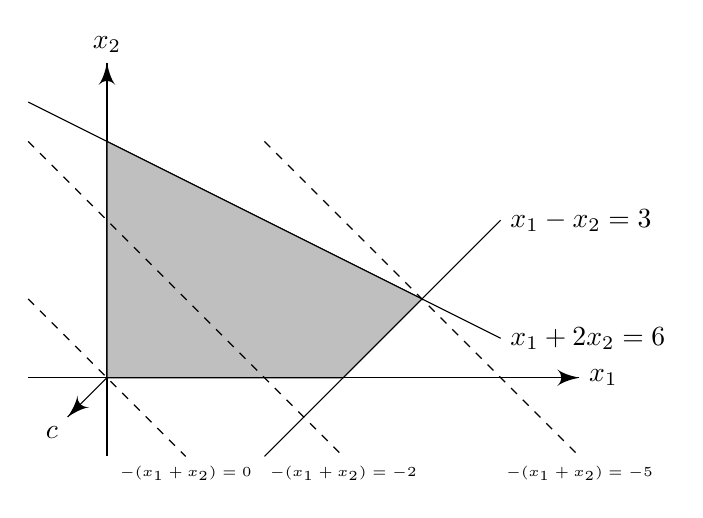
\begin{tikzpicture}
      \draw [->] (-1, 0) -- (6, 0) node [right] {$x_1$};
      \draw [->] (0, -1) -- (0, 4) node [above] {$x_2$};

      \draw (2, -1) -- (5, 2) node [right] {$x_1 - x_2 = 3$};
      \draw (-1, 3.5) -- (5, 0.5) node [right] {$x_1 + 2x_2 = 6$};
      \draw [fill=gray!50!white] (0, 0) -- (3, 0) -- (4, 1) -- (0, 3) -- cycle;
      \draw [->] (0, 0) -- (-0.5, -0.5) node [anchor=north east] {$c$};

      \draw [dashed] (-1, 1) -- (1, -1) node [below] {\tiny $-(x_1 + x_2) = 0$};
      \draw [dashed] (-1, 3) -- (3, -1) node [below] {\tiny $-(x_1 + x_2) = -2$};
      \draw [dashed] (2, 3) -- (6, -1) node [below] {\tiny $-(x_1 + x_2) = -5$};
    \end{tikzpicture}
  \end{center}
  The shaded region is the feasible region, and $c$ is our \emph{cost vector}. The dotted lines, which are orthogonal to $c$ are lines in which the objective function is constant. To minimize our objective function, we want the line to be as right as possible, which is clearly achieved at the intersection of the two boundary lines.
\end{eg}
Now we have a problem. In the general case, we have absolutely \emph{no idea} how to solve it. What we \emph{do} know, is how to do \emph{un}constrained optimization.

\subsection{Review of unconstrained optimization}
Let $f: \R^n \to \R$, $x^*\in \R^n$. A necessary condition for $x^*$ to minimize $f$ over $\R^n$ is $\nabla f(x^*) = 0$, where
\[
  \nabla  f = \left(\frac{\partial f}{\partial x_1}, \cdots, \frac{\partial f}{\partial x_n}\right)^T
\]
is the gradient of $f$.

However, this is obviously not a sufficient condition. Any such point can be a maximum, minimum or a saddle. Here we need a notion of convexity:
\begin{defi}[Convex region]
  A region $S\subseteq \R^n$ is \emph{convex} iff for all $\delta\in [0, 1]$, $x, y\in S$, we have $\delta x + (1 - \delta) y \in S$. Alternatively, If you take two points, the line joining them lies completely within the region.

  \begin{center}
    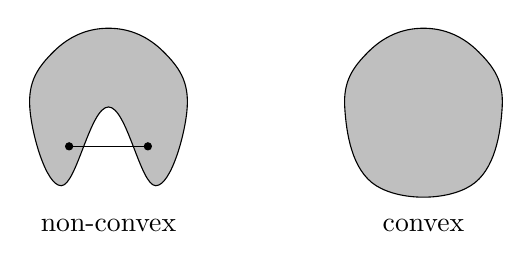
\begin{tikzpicture}
      \begin{scope}[shift={(-2, 0)}]
        \draw [fill=gray!50!white] plot [smooth cycle, tension=0.7] coordinates {(0, 1) (-0.7, 0.7) (-1, 0) (-0.6, -1) (0, 0) (0.6, -1) (1, 0) (0.7, 0.7)};
        \draw (-0.5, -0.5) node [circ] {} -- (0.5, -0.5) node [circ] {};

        \node at (0, -1.5) {non-convex};
      \end{scope}

      \begin{scope}[shift={(2, 0)}]
        \draw [fill=gray!50!white] plot [smooth cycle, tension=0.7] coordinates {(0, 1) (-0.7, 0.7) (-1, 0) (-0.6, -1) (0.6, -1) (1, 0) (0.7, 0.7)};
        \node at (0, -1.5) {convex};
      \end{scope}
    \end{tikzpicture}
  \end{center}
\end{defi}

\begin{defi}[Convex function]
  A function $f: S\to \R$ is \emph{convex} if for all $x, y\in S$, $\delta\in [0, 1]$, then $\delta f(x) + (1 - \delta)f(y) \geq f(\delta x + (1 - \delta)y)$.

  \begin{center}
    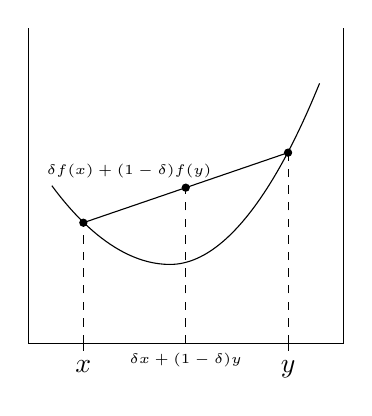
\begin{tikzpicture}
      \draw(-2, 4) -- (-2, 0) -- (2, 0) -- (2, 4);
      \draw (-1.3, 0.1) -- (-1.3, -0.1) node [below] {$x$};
      \draw (1.3, 0.1) -- (1.3, -0.1) node [below] {$y$};
      \draw (-1.7, 2) parabola bend (-.2, 1) (1.7, 3.3);
      \draw [dashed] (-1.3, 0) -- (-1.3, 1.53) node [circ] {};
      \draw [dashed] (1.3, 0) -- (1.3, 2.42) node [circ] {};
      \draw (-1.3, 1.53) -- (1.3, 2.42);
      \draw [dashed] (0, 0) node [below] {\tiny $\delta x + (1 - \delta)y$} -- (0, 1.975) node [above] {\tiny$\delta f(x) + (1 - \delta) f(y)\quad\quad\quad\quad\quad\quad$} node [circ] {};
    \end{tikzpicture}
  \end{center}

  A function is \emph{concave} if $-f$ is convex. Note that a function can be neither concave nor convex.
\end{defi}

We have the following lemma:
\begin{lemma}
  If $f$ is twice differentiable, then it is convex on a convex set $S$ if the Hessian matrix
  \[
    Hf_{ij} = \frac{\partial^2 f}{\partial x_i \partial x_j}
  \]
  is positive semidefinite on $S$, where this fancy term means:
\end{lemma}

\begin{defi}[Positive-semidefinite]
  A matrix $H$ is \emph{positive semi-definite} if $v^T Hv \geq 0$ for all $x\in S$ and $v\in \R^n$.
\end{defi}

Which leads to the following theorem:
\begin{thm}
  Let $X\subseteq \R^n$ be convex, $f: \R^n \to \R$ be twice differentiable on $X$. Let $x^* \in X$ satisfy $\nabla f(x^*) = 0$ and $Hf(x)$ is positive semidefinite for all $x\in X$. Then $x^*$ minimizes $f$ on $X$.
\end{thm}
We will not prove these.

Note that this is helpful, since linear functions are convex (and concave). The problem is that our problems are constrained, not unconstrained. So we will have to convert constrained problems to unconstrained problems.

\section{The method of Lagrange multipliers}
The trick is to include the constraints into the objective function, so that things outside the constraint will not be thought to be minima.

Suppose the problem is
\begin{center}
  minimize $f(x)$ subject to $h(x) = b$, $x\in X$.
\end{center}
Call the constraint $(P)$.
\begin{defi}[Lagrangian]
  The \emph{Lagrangian} of a constraint $(P)$ is defined as
  \[
    L(x, \lambda) = f(x) - \lambda^T(h(x) - b).
  \]
  for $\lambda\in \R^m$.
\end{defi}
Note that when the constraint is satisfied, $h(x) - b = 0$, and $L(x, \lambda) = f(x)$.

We could as well have used
\[
  L(x, \lambda) = f(x) + \lambda^T(h(x) - b).
\]
since we just have to switch the sign of $\lambda$. So we don't have to worry about getting the sign wrong.

If we minimize $L$ over both $x$ and $\lambda$, then we will magically find the minimal solution subject to the constrains. Sometimes.

\begin{thm}[Lagrangian sufficiency]
  Let $x^*\in X$ and $\lambda^*\in \R^m$ such that
  \[
    L(x^* ,\lambda^*) = \inf_{x\in X}L(x, \lambda^*)\quad\text{and}\quad h(x^*) = b.
  \]
  Then $x^*$ is optimal for ($P$).
\end{thm}
This looks like a pretty powerful result, but it turns out that it is quite easy to prove.

\begin{proof}
  We first define the ``feasible set'': let $X(b) = \{x\in X: h(x) = b\}$, ie. the set of all $x$ that satisfies the constraints. Then
  \begin{align*}
    \min_{x\in X(b)} f(x) &= \min_{x\in X(b)} (f(x) - \lambda^{*T}(h(x) - b))\quad\text{ since $h(x) - b = 0$}\\
    &\geq \min_{x\in X} (f(x) - \lambda^{*T}(h(x) - b))\\
    &= f(x^*) - \lambda^{*T}(h(x^*) - b).\\
    &= f(x^*).
  \end{align*}
\end{proof}


\begin{eg}
  Minimize $x_1 + x_2 - 2x_3$ subject to 
  \begin{align*}
    x_1 + x_2 + x_3 &= 5\\
    x_1^2 + x_2^2 = 4
  \end{align*}
  The Lagrangian is
  \begin{align*}
    L(x, \lambda) &= x_1 - x_2 - 2x_3 - \lambda_1(x_1 + x_2 + x_3 - 5) - \lambda_2 (x_1^2 + x_2^2 - 4)\\
    &= ((1 - \lambda_1)x_1 - 2\lambda_2 x_1^2) + ((-1 - \lambda_1)x_2 - \lambda_2 x_2^2) \\
    &+ (-2 - \lambda_1)x_3 + 5\lambda_1 + 4\lambda_2
  \end{align*}
  We want to pick a $\lambda^*$ and $x^*$ such that $L(x^*, \lambda^*)$ is minimal. Then for our $\lambda^*$, $L(x, \lambda^*)$  must have a finite minimum!

  We note that $(-2 - \lambda_1)x_3$ does not have a finite minimum unless $\lambda_1 = -2$. Also, the terms in $x_1$ and $x_2$ do not have a finite minimum unless $\lambda_2 < 0$.

  With these in mind, we find a minimum by setting all first derivatives to be $0$:
  \begin{align*}
    \frac{\partial L}{\partial x_1} &= 1 - \lambda_1 - 2\lambda_2 x_1 = 3 - 2\lambda_2x_1\\
    \frac{\partial L}{\partial x_1} &= -1 - \lambda_1 - 2\lambda_2 x_2 = 1 - 2\lambda_2 x_2
  \end{align*}
  Since these must be both $0$, we must have
  \[
    x_1 = \frac{3}{2\lambda_2}, \quad x_2 = \frac{1}{2\lambda_2}.
  \]
  To show that this is indeed a minimum, we look at the Hessian matrix:
  \[
    HL =
    \begin{pmatrix}
      -2\lambda_2 & 0\\
      0 & -2\lambda_2
    \end{pmatrix}
  \]
  which is positive semidefinite when $\lambda_2 < 0$, which is the condition we came up with at the beginning.

  Let $Y = \{\lambda: \R^2: \lambda_1 = -2, \lambda_2 < 0\}$ be our helpful values of $\lambda$.

  So we have shown above that for every $\lambda \in Y$, $L(x, \lambda)$ has a unique minimum at $x(\lambda) = (\frac{3}{2\lambda_2}, \frac{1}{2\lambda2}, x_3)^T$.

  Now all we have to do is find $\lambda$ and $x$ such that $x(\lambda)$ satisfies the functional constraints. The second constraint gives
  \[
    x_1^2 + x_2^2 = \frac{9}{4\lambda^2} + \frac{1}{4\lambda_2^2} = 4 \Leftrightarrow \lambda_2 = -\sqrt{\frac{5}{8}}.
  \]
  The first constraint gives
  \[
    x_3 = 5 - x_1 - x_2.
  \]
  So the theorem implies that
  \[
    x_1 = -3\sqrt{\frac{2}{5}},\quad x_2 = -\sqrt{\frac{2}{5}},\quad x_3 = 5 + 4\sqrt{\frac{2}{5}}.
  \]
\end{eg}
So far so good. But what if our functional constraint is an inequality? We will need slack variables.

To minimize $f(x)$ subject to $h(x) \leq b$, $x\in X$, we proceed as follows:
\begin{enumerate}
  \item Introduce slack variables to obtain the equivalent problem, to minimize $f(x)$ subject to $h(x) + z = b$, $x \in X$, $z \geq 0$.
  \item Compute the Lagrangian
    \[
      L(x, z, \lambda) = f(x) - \lambda^T(f(x) + z - b).
    \]
  \item Find $Y = \{\lambda: \inf_{x\in X, z\geq 0}L(x, z, \lambda) > -\infty\}$.
  \item For each $\lambda\in Y$, minimize $L(x, z, \lambda)$, ie. find
    \[
      x^*(\lambda)\in X,\quad z^*(\lambda) \geq 0
    \]
    such that
    \[
      L(x^*(\lambda), z^*(\lambda), \lambda) = \inf_{x\in X, z\geq 0} L(x, z, \lambda)
    \]
  \item Find $\lambda^*\in Y$ such that 
    \[
      h(x^*(\lambda^*)) + z^*(\lambda^*) = b.
    \]
\end{enumerate}
Then by the Lagrangian sufficiency condition, $x^*(\lambda^*)$ is optimal for the constrained problem.

\subsection{Complementary Slackness}
If we introduce a slack variable $z$, we note that $z_j$ can be made arbitrarily large in magnitude. We don't want it to be able to become arbitrarily negative, because we need a finite minimum. So we want $\lambda_j z_j$ to be always positive. So $\lambda\in Y$ requires either that $\lambda_j \geq 0$ or $\lambda_j \leq 0$, depending on the sign of $z_j$ and $b_j$.

We can get a stronger result - for every $\lambda\in Y$ and $j = 1, \cdots, m$,
\begin{align*}
  (z^*(\lambda))_j \not= 0 &\Rightarrow \lambda_j = 0\\
  \lambda_j \not= 0 &\Rightarrow (z^*(\lambda))_j = 0.
\end{align*}
This can be phrased as ``exactly one of $(z^*(\lambda))_j$ and $\lambda_j$ is $0$''.

This is due to the minimality of $z^*(\lambda)$. If $\lambda_j, z_j \not= 0$, then by making $z^*_j$ slightly smaller in magnitude, $\lambda_j z_j$ can get smaller.

If we don't want slack variables, we can write this as
\begin{align*}
  (h(x^*(\lambda^*)))_j > b_j &\Rightarrow \lambda_j^* = 0\\
 \lambda_j^* > 0 &\Rightarrow (h(x^*(\lambda^*)))_j = b_j.
\end{align*}
This makes our life easier since our search space is smaller.

\begin{eg}
  Consider the following problem:
  \begin{center}
    maximize $x_1 - 3x_2$ subject to
    \begin{align*}
      x_1^2 + x_2^2 + z_1 &= 4\\
      x_1 + x_2 + z_2 + z_2 &= 2\\
      z_1, z_2 &\geq 0.
    \end{align*}
  where $z_1, z_2$ are slack variables.
  \end{center}

  The Lagrangian is
  \[
    L(x, z, \lambda) = ((1 - \lambda_2)x_1 - \lambda_1 x_1^2) + ((-3 - \lambda_2)x_2 - \lambda_1 x_2^2) - \lambda_1 z_1 - \lambda_2 z_2 + 4\lambda_1 + 2\lambda_2.
  \]
  To ensure finite minimum, we need $\lambda_1, \lambda_2 \leq 0$.

  By complementary slackness, $\lambda_1 z_1 = \lambda_2 z_2 = 0$. We can then consider the cases $\lambda_1 = 0$ and $z_1 = 0$ separately, and save a lot of algebra.
\end{eg}

\section{Shadow prices and Lagrange Duality}
\subsection{Shadow prices}
Let
\[
  \phi(b) = \inf \{f(x): h(x) = b, x\in X\}.
\]
Note that this allows infinite values of $\phi$. If there is no $x$ that satisfies $h(x) = b, x\in X$, then the infimum is positive infinity. If $f(x)$ can be unboundedly small, then $\phi(b) = -\infty$.

\begin{thm}[]
  Suppose $f$ and $h$ are continuously differentiable on $\R^n$, and that there exist unique functions $x^*: \R^m \to \R^n$, $\lambda^*: \R^m \to \R^n$ ($m$ is the dimension of $b$, $n$ is the dimension of $x$), such that for each $b\in \R^m$, 
  \[
    \lambda^*(b) \geq 0 \text{ and } f(x^*(b)) = \phi(b).
  \]
  If $x^*$ and $\lambda^*$ are continuously differentiable, then for $i = 1, \cdots, m$, we have
  \[
    \frac{\partial \phi}{\partial b_i}(b) = \lambda_i^*(b).
  \]
\end{thm}
$\frac{\partial \phi}{\partial b_i}$ should be interpreted as follows: think of $b$ as the total amount of resources we have, and $h(x)$ is the amount of resources we need if we produce $x$ many goods. Then $\frac{\partial \phi}{\partial b_i}$ is how much more we will be able to produce when our available resources change.

Proof is omitted, as it is just a tedious application of chain rule etc.

The result also holds when the functional constraints are inequality constraints: if the $i$th constraint at an optimal solution does not hold with equality, then the Lagrange multiplier is $0$ by complementary slackness. Also, the partial derivative of $\phi$ with respect to $b_i$ also has to be $0$, since changing the upper bound doesn't affect us if we are not at the limit.
\subsection{Lagrange duality}
Suppose the problem is
\begin{center}
  minimize $f(x)$ subject to $h(x) = b$, $x\in X$.
\end{center}
Denote this as $D$.

The Lagrangian is
\[
  L(x, \lambda) = f(x) - \lambda^T (h(x) - b).
\]
Define the dual function $g: \R^m \to \R$ as
\[
  g(\lambda) = \inf_{x\in X}L(x, \lambda).
\]
ie, if we fix $\lambda$, how small we can get $L$ to be. As before, let
\[
  Y = \{\lambda\in \R^n: g(\lambda) > -\infty\}.
\]
Then we have
\begin{thm}[Weak duality]
  If $x\in X(b)$ (ie. $x$ satisfies both the functional and regional constraints) and $\lambda \in Y$, then
  \[
    g(\lambda) \leq f(x).
  \]
  In particular,
  \[
    \sup_{\lambda\in Y}g(\lambda) \leq \inf_{x\in X(b)}f(x).
  \]
\end{thm}

\begin{proof}
  \begin{align*}
    g(\lambda) &= \inf_{x'\in X}L(x', \lambda)\\
    &\leq L(x, \lambda)\\
    &= f(x) - \lambda^T (h(x) - b)\\
    &= f(x).
  \end{align*}
\end{proof}

This suggests that we can solve a dual problem - instead of minimizing $f$, we can maximize $g$ subject to $\lambda\in Y$. Denote this problem as $(D)$. The original problem $(P)$ is called \emph{primal}.

\begin{defi}[Strong duality]
  $(P)$ and $(D)$ are said to satisfy \emph{strong duality} if
  \[
    \sup_{\lambda\in Y}g(\lambda) = \inf_{x\in X(b)}f(x).
  \]
\end{defi}
It turns out that problems satisfying strong duality are exactly those for which the method of Lagrange multipliers work.

\begin{eg}
  Again consider the problem to minimize $x_1 - x_2 - 2x_3$ subject to
  \begin{align*}
    x_1 + x_2 + x_3 &= 5\\
    x_1^2 + x_2^2 &= 4
  \end{align*}
  We saw that 
  \[
    Y = \{\lambda\in \R^2: \lambda_1 = -2, \lambda_2 < 0\}
  \]
  and
  \[
    x^*(\lambda) = \left(\frac{3}{2\lambda_2}, \frac{1}{2\lambda_2}, 5 - \frac{4}{2\lambda_2}\right).
  \]
  The dual function is
  \[
    g(\lambda) = \inf_{x\in X} L(x, \lambda) = L(x^*(\lambda), \lambda) = \frac{10}{4\lambda_2} + 4\lambda_2 - 10.
  \]
  The dual is the problem to
  \begin{center}
    maximize $\frac{10}{4\lambda_2} + 4\lambda_2 - 10$ subject to $\lambda_2 < 0$.
  \end{center}

  The maximum is attained for
  \[
    \lambda_2 = -\sqrt{\frac{5}{8}}.
  \]
  So the primal and dual have the same optimum value.
\end{eg}

Right now, what we've got isn't helpful, because we won't know if our problem satisfies strong duality!

\section{Conditions for strong duality}
\subsection{Supporting hyperplanes and convexity}
Consider
\[
  \phi(b) = \inf\{f(x): h(x) = b, x\in X\}.
\]
Fix $b\in \R^m$ and consider $\phi(c)$ as a function $c\in \R^m$. Further consider the hyperplane given by $\lambda: \R^m \to \R$ where $\alpha(c) = \beta + \lambda^T(c - b)$.

\begin{center}
  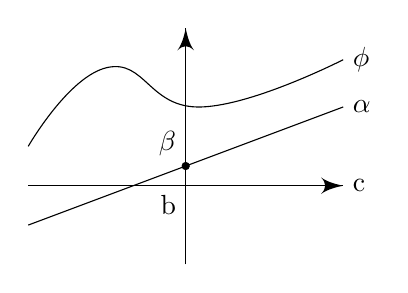
\begin{tikzpicture}
    \draw [->] (-2, 0) -- (2, 0) node [right] {c};
    \draw [->] (0, -1) -- (0, 2);
    \node [anchor = north east] {b};
    \draw plot [smooth, tension=0.8] coordinates {(-2, 0.5) (-1, 1.5) (0.2, 1) (2, 1.6)} node [right] {$\phi$};
    \draw (-2, -0.5) -- (2, 1) node [right] {$\alpha$};
    \node [circ] at (0, 0.25) {};
    \node [anchor = south east] at (0, 0.25) {$\beta$};
  \end{tikzpicture}
\end{center}

We can try to determine $\phi(b)$ as follows:
\begin{enumerate}
  \item For each $\lambda$ (slope of line $\alpha$), find 
    \[
      \beta_\lambda = \max \{\beta: \beta + \lambda^T(c - b) \leq \phi(c)\text{ for all }c\}
    \]
    ie. we push up the line as far as possible while remaining below $\phi(c)$.
  \item Choose $\lambda$ to maximize $\beta_\lambda$. This is what maximizes the dual function $g(\lambda)$.
\end{enumerate}
We see weak duality as $\max_\lambda \beta_\lambda \leq \phi(b)$.

\begin{defi}[Supporting hyperplane]
  A hyperplane $\alpha: \R^m \to \R$ is \emph{supporting} to $\phi$ at $b$ if for all $c$, $\alpha(c) = \phi(b) + \lambda^T(c - b)$, ie. $\beta = \phi(b)$, and $\phi(c) \geq \alpha(c)$ for all $c$.

  \begin{center}
    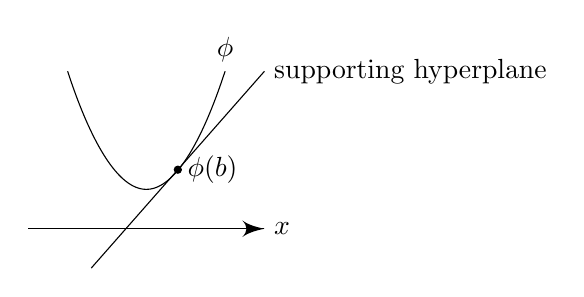
\begin{tikzpicture}
      \draw [->] (-1.5, 0) -- (1.5, 0) node [right] {$x$};
      \draw (-1, 2) parabola bend (0, 0.5) (1, 2) node [above] {$\phi$};
      \node [circ] at (0.4, 0.75) {};
      \node [right] at (0.4, 0.75) {$\phi(b)$};
      \draw (-0.7, -0.5) -- (1.5, 2) node [right] {supporting hyperplane};
    \end{tikzpicture}
  \end{center}
\end{defi}

\begin{thm}[]
  $(P)$ satisfies strong duality iff there exists a supporting hyperplane at $b$.
\end{thm}

\begin{proof}
  $(\Leftarrow)$ Suppose there is a supporting hyperplane. Then by definition there exists $\lambda\in \R^m$ such that for all $c\in \R^m$,
  \[
    \phi(b) + \lambda^T(c - b) \leq \phi(c).
  \]
  This implies that
  \begin{align*}
    \phi(b) &\leq \inf_{c\in \R^m}(\phi(c) - \lambda^T(c - b))\\
    &= \inf_{c\in \R^m}\inf_{x\in X(c)}(f(x) - \lambda^T(h(x) - b))\\
    \intertext{Since $\phi(c) = \inf_{x\in X(c)} f(x)$ and $h(x) = c$ for $x\in X(c)$}
    &= \inf_{x\in X}L(x, \lambda).\\
    \intertext{since $\bigcup_{c\in \R^m}X(c) = X$, which is true since for any $x\in X$, we have $x\in X(h(x))$.}
    &= g(\lambda)
  \end{align*}
  By weak duality, $g(\lambda) \leq \phi(b)$. So $\phi(b) = g(\lambda)$. So strong duality holds.

  $(\Rightarrow)$. Assume now that we have strong duality. The there exists $\lambda$ such that for all $c\in \R^m$,
  \begin{align*}
    \phi(b) &= g(\lambda)\\
    &= \inf_{x\in X}L(x, \lambda)\\
    &\leq \inf_{x\in X(c)} L(x, \lambda)\\
    &= \inf_{x\in X(c)} (f(x) - \lambda^T(h(x) - b))\\
    &= \phi(c) - \lambda^T(c - n)
  \end{align*}
  So $\phi(b) + \lambda^T(c - b) \leq \phi(c)$. So this defines a supporting hyperplane.
\end{proof}

\begin{thm}[Supporting hyperplane theorem]
  Suppose that $\phi: \R^m \to \R$ is convex and $b\in\R^m$ lies in the interior of the set of points where $\phi$ is finite. Then there exists a supporting hyperplane to $\phi$ at $b$.
\end{thm}

This is still not helpful, since we don't know what $\phi$ is! So now we have a sufficient condition for Lagrange multipliers to work:
\subsection{A sufficient condition for convexity of \texorpdfstring{$\phi$}{phi}}
\begin{thm}[]
  Let 
  \[
    \phi(b) = \inf_{x} \{f(x): h(x) \leq b, x\in X\}
  \]
  Then $\phi$ is convex if $X, f, h$ are convex, assuming feasibility and boundedness.
\end{thm}

\begin{proof}
  Consider $b_1, b_2\in \R^m$ such that $\phi(b_1)$ and $\phi(b_2)$ are defined. Let $\delta \in [0, 1]$ and define $b = \delta b_1 + (1 - \delta)b_2$. We want to show that $\phi(b) \leq \delta \phi(b_1) + (1 - \delta)\phi(b_2)$.

  Consider $x_1 \in X(b_1)$, $x_2 \in X(b_2)$, and let $x = \delta x_1 + (1 - \delta)x_2$. By convexity of $X$, $x\in X$.

  By convexity of $h$,
  \begin{align*}
    h(x) &= h(\delta x_1 + (1 - \delta) x_2)\\
    &\leq \delta h(x_1) + (1 - \delta)h(x_2)\\
    &\leq \delta b_1 + (1 - \delta)b_2\\
    &= b
  \end{align*}
  So $x\in X(b)$. Since $\phi(x)$ is an optimal solution, by convexity of $f$, 
  \begin{align*}
    \phi(b) &\leq f(x)\\
    &= f(\delta x_1 + (1 - \delta x_2))\\
    &\leq \delta f(x_1) + (1 - \delta)f(x_2)
   \end{align*}
   This holds for any $x_1\in X(b_1)$ and $x_2 \in X(b_2)$. So by taking infimum of the right hand side,
   \[
     \phi(b) \leq \delta \phi(b_1) + (1 - \delta) \phi(b_2).
   \]
   So $\phi$ is convex.
\end{proof}
$h(x) = b$ is equivalent to $h(x) \leq b$ and $-h(x) \leq -b$. So the result holds for problems with equality constraints if both $h$ and $-h$ are convex, ie. if $h(x)$ is linear.

So
\begin{thm}[]
  If a linear program is feasible and bounded, then it satisfies strong duality.
\end{thm}

\section{Solutions of linear programs}

\end{document}
